\documentclass[tikz]{standalone}
\usepgflibrary{arrows.meta}
\usepackage{xcolor}
\begin{document}
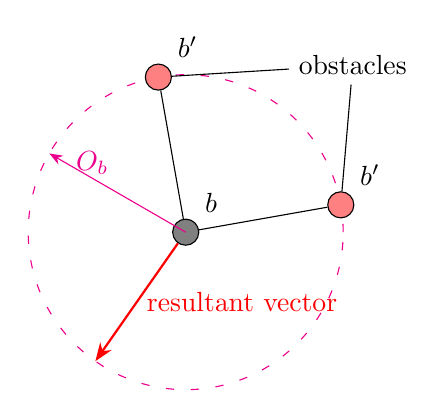
\begin{tikzpicture}[>=Stealth]
	\node[circle,fill=black!50,draw,label=above right:$b$](b){};


  \draw[loosely dashed,radius=2cm,draw=magenta] (0,0) circle;
  \draw[->,magenta] (0,0)-- node[very near end,right]{$O_b$} (150:2cm) ;
  
  \draw (100:2cm) node[circle,fill=red!50,draw,label=above right:$b'$](b0){};
  \draw (10:2cm) node[circle,fill=red!50,draw,label=above right:$b'$](b1){};

  \draw (b) edge (b0);
  \draw (b) edge (b1);

  \draw[thick,red,->] (b) -- node[right]{resultant vector} (235:2cm);

  \draw (45:3cm) node (p) {obstacles};
  \draw (p) edge (b0);
  \draw (p) edge (b1);
\end{tikzpicture}
\end{document}

